\begin{columns}
    \begin{column}[t]{0.7\textwidth}
        Given are
        \begin{itemize}
            \item graph $G=(V,E)$
            \item one position $(n_x,n_y)$ inside unit square for each node $n\in V$
            \item small stripes at the edges of the unit square
        \end{itemize}
        $G$ is called percolating, if there are nodes $n,m\in V$ such that
        \begin{enumerate}
            \item there is a cycle containing $n$ and $m$
            \item $n$ are connected by an edge
            \item $n$ and $m$ lie in opposite stripes
        \end{enumerate}
    \end{column} 
    \begin{column}[t]{0.3\textwidth}
        \vspace{-1cm}
        \begin{figure}[t]
            \centering
            %\hfill
            \begin{subfigure}{\textwidth}
                \centering
                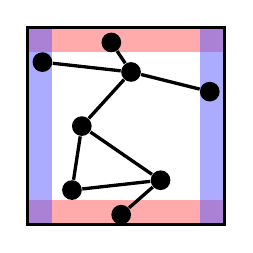
\begin{tikzpicture}[
                    node/.style={circle, inner sep=0pt, fill=black, minimum size=2.5mm}
                ]
                \useasboundingbox[fill=white](0,0) rectangle(0.625*4,0.625*4);
                \fill[red!65, fill opacity=0.5] (0,0) rectangle (0.625*4, 0.625*0.5);
                \fill[red!65, fill opacity=0.5] (0,0.625*3.5) rectangle (0.625*4, 0.625*4);
                \fill[blue!65, fill opacity=0.5] (0,0) rectangle (0.625*0.5, 0.625*4);
                \fill[blue!65, fill opacity=0.5] (0.625*3.5,0) rectangle (0.625*4, 0.625*4);
                \draw[black, very thick] (0,0) rectangle (0.625*4,0.625*4);
                \node[node] at (0.625*0.3, 0.625*3.3) (n1) {};
                \node[node] at (0.625*1.1, 0.625*2.0) (n2) {};
                \node[node] at (0.625*0.9, 0.625*0.7) (n3) {};
                \node[node] at (0.625*2.7, 0.625*0.9) (n4) {};
                \node[node] at (0.625*2.1, 0.625*3.1) (n5) {};
                \node[node] at (0.625*3.7, 0.625*2.7) (n6) {};
                \node[node] at (0.625*1.7, 0.625*3.7) (n7) {};
                \node[node] at (0.625*1.9, 0.625*0.2) (n8) {};
                \draw[very thick]  (n1) -- (n5);
                \draw[very thick]  (n5) -- (n2);
                \draw[very thick]  (n5) -- (n6);
                \draw[very thick]  (n2) -- (n4);
                \draw[very thick]  (n3) -- (n4);
                \draw[very thick]  (n2) -- (n3);
                \draw[very thick]  (n5) -- (n7);
                \draw[very thick]  (n8) -- (n4);
                \end{tikzpicture}
                \caption{non-percolating}
            \end{subfigure}
            \par\bigskip
            \begin{subfigure}{\textwidth}
                \centering
                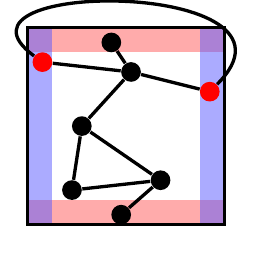
\begin{tikzpicture}[
                    node/.style={circle, inner sep=0pt, fill=black, minimum size=2.5mm},
                    node_c/.style={circle, inner sep=0pt, fill=red, minimum size=2.5mm}
                ]
                \useasboundingbox[fill=white](0,0) rectangle(0.625*4,0.625*4);
                \fill[red!65, fill opacity=0.5] (0,0) rectangle (0.625*4, 0.625*0.5);
                \fill[red!65, fill opacity=0.5] (0,0.625*3.5) rectangle (0.625*4, 0.625*4);
                \fill[blue!65, fill opacity=0.5] (0,0) rectangle (0.625*0.5, 0.625*4);
                \fill[blue!65, fill opacity=0.5] (0.625*3.5,0) rectangle (0.625*4, 0.625*4);
                \draw[black, very thick] (0,0) rectangle (0.625*4,0.625*4);
                \node[node_c] at (0.625*0.3, 0.625*3.3) (n1) {};
                \node[node] at (0.625*1.1, 0.625*2.0) (n2) {};
                \node[node] at (0.625*0.9, 0.625*0.7) (n3) {};
                \node[node] at (0.625*2.7, 0.625*0.9) (n4) {};
                \node[node] at (0.625*2.1, 0.625*3.1) (n5) {};
                \node[node_c] at (0.625*3.7, 0.625*2.7) (n6) {};
                \node[node] at (0.625*1.7, 0.625*3.7) (n7) {};
                \node[node] at (0.625*1.9, 0.625*0.2) (n8) {};
                \draw[very thick]  (n1) -- (n5);
                \draw[very thick]  (n5) -- (n2);
                \draw[very thick]  (n5) -- (n6);
                \draw[very thick]  (n2) -- (n4);
                \draw[very thick]  (n3) -- (n4);
                \draw[very thick]  (n2) -- (n3);
                \draw[very thick]  (n5) -- (n7);
                \draw[very thick]  (n8) -- (n4);
                \draw[very thick]  (n1) .. controls (-0.625*2,0.625*5) and (0.625*6,0.625*5) .. (n6);
                \end{tikzpicture}
                \caption{percolating}
            \end{subfigure}
        \end{figure}   
        \vfill     
    \end{column}   
\end{columns}